\chapter{Transformacja Hough'a}
\label{sec:hough}

Transformacja Hough'a (czyt. Haf'a) wykorzystywana jest w~procesie analizy obrazów i~służy do wykrywania na nim kształtów parametrycznych oraz nieparametrycznych w~zależności od jej wariantu \cite{mukhopadhyay2015survey}. Samo pojęcie transformacji odnosi się do odwzorowywania pojedynczych pikseli obrazu binarnego lub ich zbioru w~przestrzeni akumulatora. Obraz wejściowy wcześniej poddany być musi procesowi wykrywania krawędzi. Dane zebrane w~akumulatorze biorą następnie udział w~procesie głosowania, w~którym wyłonieni zostają potencjalne kształty poprzez wykrywanie największych wartości w~akumulatorze. W~zależności od specyfiki problemu oraz wykrywanych kształtów głosowanie nad kandydatami może odbywać się na różne sposoby. Użyte może zostać proste progowanie, wykrywanie i~uśrednianie skupisk, czy też filtracja przestrzeni akumulatora. Ogólny schemat przetwarzania przedstawiony jest na rysunku \ref{fig:hough}.

\begin{figure}
    \centering
    \begin{tikzpicture}


\node[draw, rectangle, minimum height=0.9cm] (e) {Edge detection};
\node[draw, rectangle, minimum height=0.9cm, right=0.9cm of e] (t) {Hough transform};
\node[draw, rectangle, minimum height=0.9cm, right=0.9cm of t] (v) {Voting};
\node[draw, rectangle, minimum height=0.9cm, right=0.9cm of v] (p) {Further processing};

\path [draw, latex-o, ultra thick] (e) -- node[right] {Input image} ++(0,2);
\path [draw, -latex, ultra thick] (e) -- node[right] {} (t);
\path [draw, -latex, ultra thick] (t) -- node[right] {} (v);
\path [draw, -latex, ultra thick] (v) -- node[right] {} (p);
\path [draw, -latex, ultra thick] (p) -- node[left] {Detected patterns} ++(0,2);

\end{tikzpicture}

    \caption{Ogólny schemat przetwarzania obrazu z wykorzystaniem transformacji Hough'a.}
    \label{fig:hough}
\end{figure}

\section{Standard Hough Transform}

Pracą, która jako pierwsza opisała tę transformację jest zgłoszony w~1962r. patent Paula Hough'a. Opisał on wykrywanie linii poprzez zastosowanie odwzorowania PTLM (point-to-line mapping). Odwzorowanie to dla każdego piksela rysuje linię w~dwuwymiarowej przestrzeni akumulatora zgodnie z kierunkowym równaniem prostej z~równania (\ref{eq:hough-1}) przekształcone do postaci (\ref{eq:hough-2}). Stosując odwzorowanie odwrotne dla punktów o~największych wartościach możemy otrzymać potencjalne linie na obrazie.
\begin{align}
    y &= mx+c \label{eq:hough-1}\\
    c &= y-mx \label{eq:hough-2}
\end{align}
\begin{eqexpl}
    \item{x, y} współrzędne piksela na obrazie;
    \item{m} zbocze prostej;
    \item{c} punkt przecięcia prostej.
\end{eqexpl}


% \begin{figure}
%     \centering
%     \begin{tikzpicture}[scale=0.9]
    \begin{scope}[yscale=-1] 
    \tkzInit[xmax=6.2,ymax=6.2,xmin=0,ymin=0]
    \tkzGrid[]
    \tikzset{xlabel style/.append style={above=5pt}}
    \tkzAxeXY[]
    \draw[gray, ultra thick] (-0.5,0.5) -- (5.5,6.5);
    \fill (0, 1)  circle[radius=2pt];
    \fill (1, 2)  circle[radius=2pt];
    \fill (2, 3)  circle[radius=2pt];
    \fill (3, 4)  circle[radius=2pt];
    \fill (4, 5)  circle[radius=2pt];
    \fill (5, 6)  circle[radius=2pt];
    \end{scope}
\end{tikzpicture}

%     \caption{Ogólny schemat przetwarzania obrazu z wykorzystaniem transformacji Hough'a.}
%     \label{fig:houghSlopeA}
% \end{figure}

\begin{figure}
    \centering
    \begin{subfigure}{0.4\textwidth}
        \centering
        \begin{tikzpicture}[scale=0.9]
    \begin{scope}[yscale=-1] 
    \tkzInit[xmax=6.2,ymax=6.2,xmin=0,ymin=0]
    \tkzGrid[]
    \tikzset{xlabel style/.append style={above=5pt}}
    \tkzAxeXY[]
    \draw[gray, ultra thick] (-0.5,0.5) -- (5.5,6.5);
    \fill (0, 1)  circle[radius=2pt];
    \fill (1, 2)  circle[radius=2pt];
    \fill (2, 3)  circle[radius=2pt];
    \fill (3, 4)  circle[radius=2pt];
    \fill (4, 5)  circle[radius=2pt];
    \fill (5, 6)  circle[radius=2pt];
    \end{scope}
\end{tikzpicture}

    \caption{Binarny obraz wejściowy}\label{fig:houghSlopeA}
    \end{subfigure}
    \begin{subfigure}{0.4\textwidth}
        \centering
        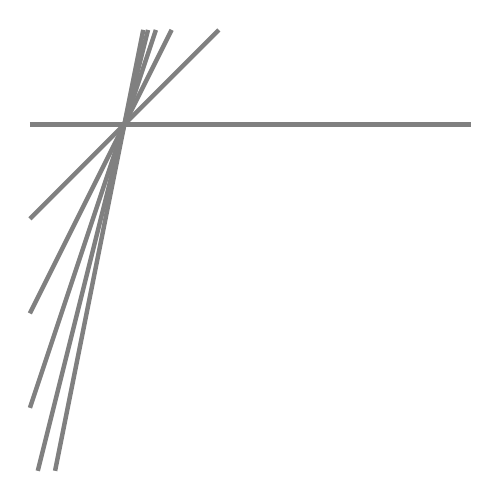
\begin{tikzpicture}[scale=0.8]
    \begin{scope}[yscale=-1] 
    \tkzInit[xmax=6,ymax=6,xmin=0,ymin=0]
    \tkzGrid[]
    \tikzset{xlabel style/.append style={above=5pt}}
    \tkzAxeXY[]
    \draw[gray, ultra thick] (-0.5,1) -- (6.5,1);
    \draw[gray, ultra thick] (-0.5,2.5) -- (2.5,-0.5);
    \draw[gray, ultra thick] (-0.5,4) -- (1.75,-0.5);
    \draw[gray, ultra thick] (-0.5,5.5) -- (1.5,-0.5);
    \draw[gray, ultra thick] (-0.375,6.5) -- (1.375,-0.5);
    \draw[gray, ultra thick] (-0.1,6.5) -- (1.3,-0.5);
    \end{scope}
\end{tikzpicture}

    \caption{Wynik transformacji}\label{fig:houghSlopeB}
    \end{subfigure}

    \caption{Demonstracja transformacji Hough'a w wariancie równania kierunkowego prostej.}
\end{figure}

\begin{figure}
    \centering
    \begin{tikzpicture}[]
    \tkzInit[xmax=360,xstep=30,ymax=3,xmin=0,ymin=-3]
    \tkzGrid[]
    \tkzClip[space=0.75]
    \tkzDrawX[label=$\theta$]
    \tkzLabelX
    \tkzDrawY[label=$\rho$]
    \tkzLabelY

    \draw plot[domain=0:360/30,smooth] (\x,{0*cos(\x*30*0.0174532925 r) + 1*sin(\x*30*0.0174532925 r)});
    \draw plot[domain=0:360/30,smooth] (\x,{1*cos(\x*30*0.0174532925 r) + 2*sin(\x*30*0.0174532925 r)});
    \draw plot[domain=0:360/30,smooth] (\x,{2*cos(\x*30*0.0174532925 r) + 3*sin(\x*30*0.0174532925 r)});
    \draw plot[domain=0:360/30,smooth] (\x,{3*cos(\x*30*0.0174532925 r) + 4*sin(\x*30*0.0174532925 r)});
    \draw plot[domain=0:360/30,smooth] (\x,{4*cos(\x*30*0.0174532925 r) + 5*sin(\x*30*0.0174532925 r)});
    \draw plot[domain=0:360/30,smooth] (\x,{5*cos(\x*30*0.0174532925 r) + 6*sin(\x*30*0.0174532925 r)});
\end{tikzpicture}

    \caption{Wynik transformacji Hough'a dla obrazu na rysunku \ref{fig:houghSlopeA} w wariancie współrzędnych biegunowych.}
    \label{fig:houghSinCos}
\end{figure}

\section{Circle Hough Transform}

